%%% ===== In the main body, replace the old §4–§7 figure blocks with: =====

\section{Epoch‐Budget Ablation}
We observe extreme overfitting within $\sim$15 epochs and noisy validation spikes (see App.~A).  % trimmed discussion

\section{Negative‐Sampling Hardness}
Figure~\ref{fig:neg-sampling} shows validation‐only curves: dense negatives (solid) converge smoothly to $\sim$0.82 accuracy, whereas random negatives collapse toward 1.0 then oscillate $\pm$0.1, risking unstable checkpoints.
\begin{figure}[t]
  \centering
  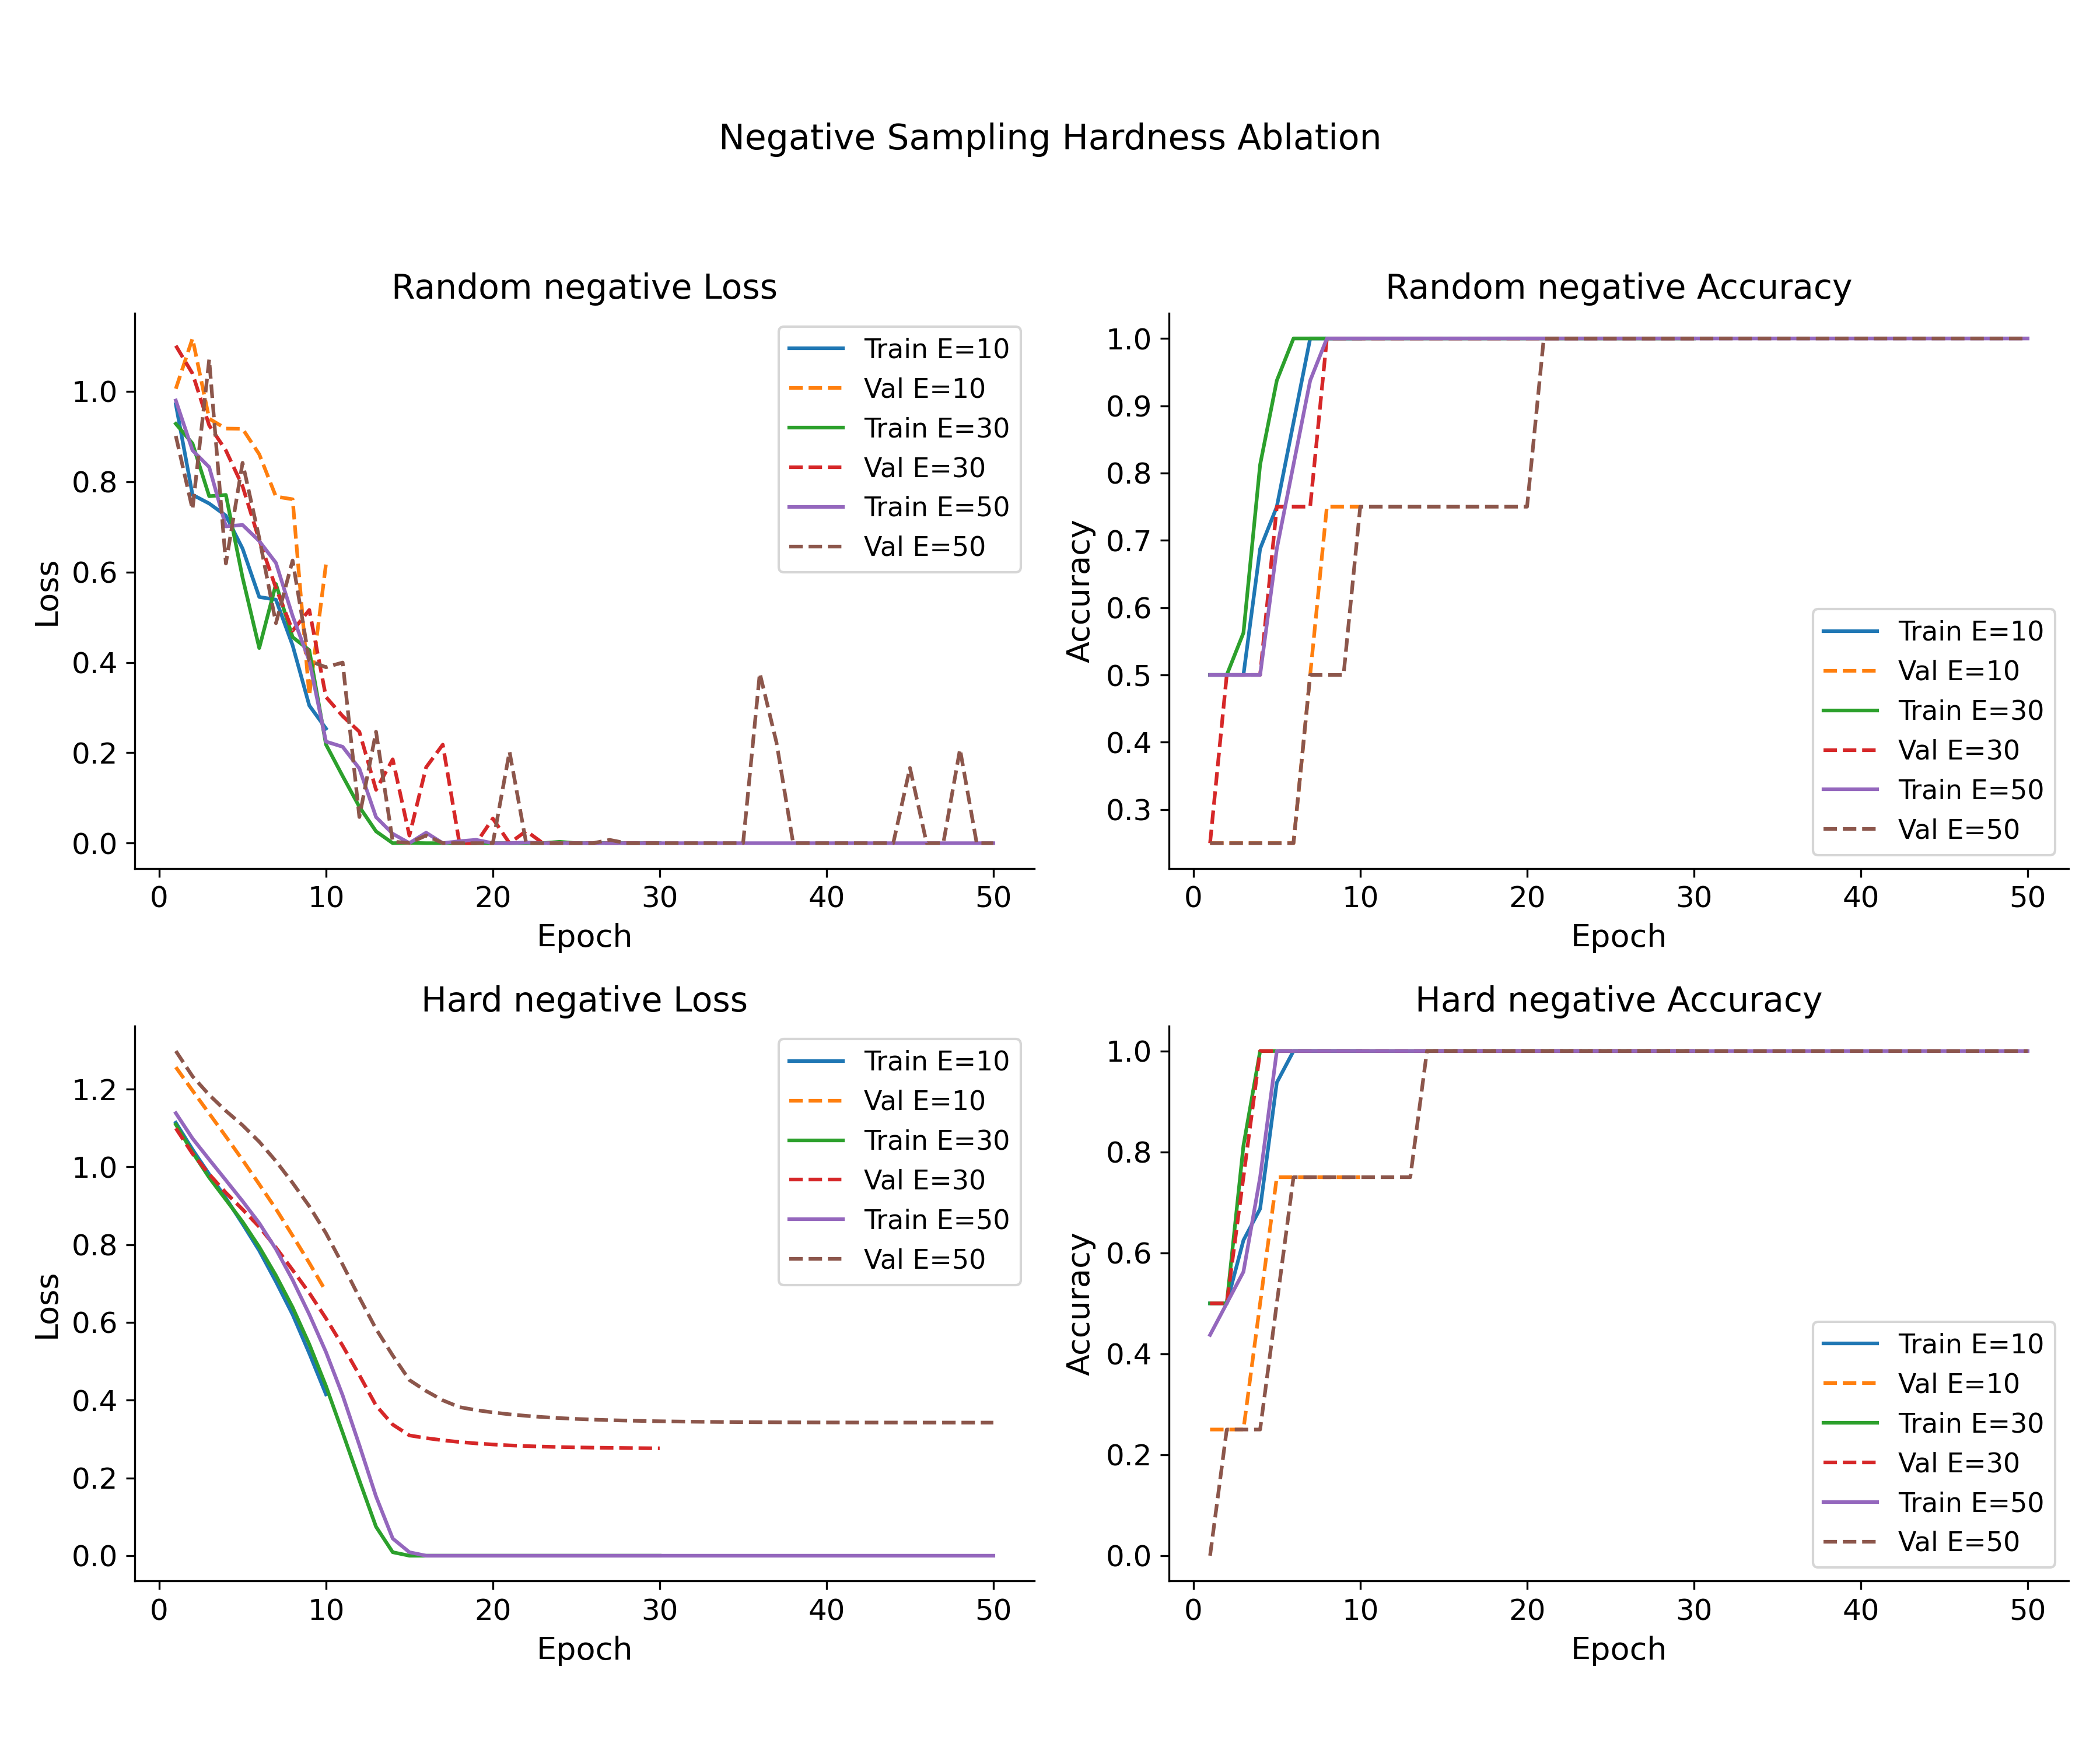
\includegraphics[width=0.9\linewidth]{negative_sampling_hardness.png}
  \caption{Validation curves for hard vs.\ random negative sampling. Random negatives induce large oscillations.}
  \label{fig:neg-sampling}
\end{figure}

\section{Distance Metric Ablation}
Figure~\ref{fig:dist-metric} isolates validation performance at $E=30$: Euclidean yields $<0.02$ loss‐variance and 0.99$\pm$0.005 accuracy after 10 epochs; cosine shows $>0.05$ variance and only reaches 0.95 by epoch 30.
\begin{figure}[t]
  \centering
  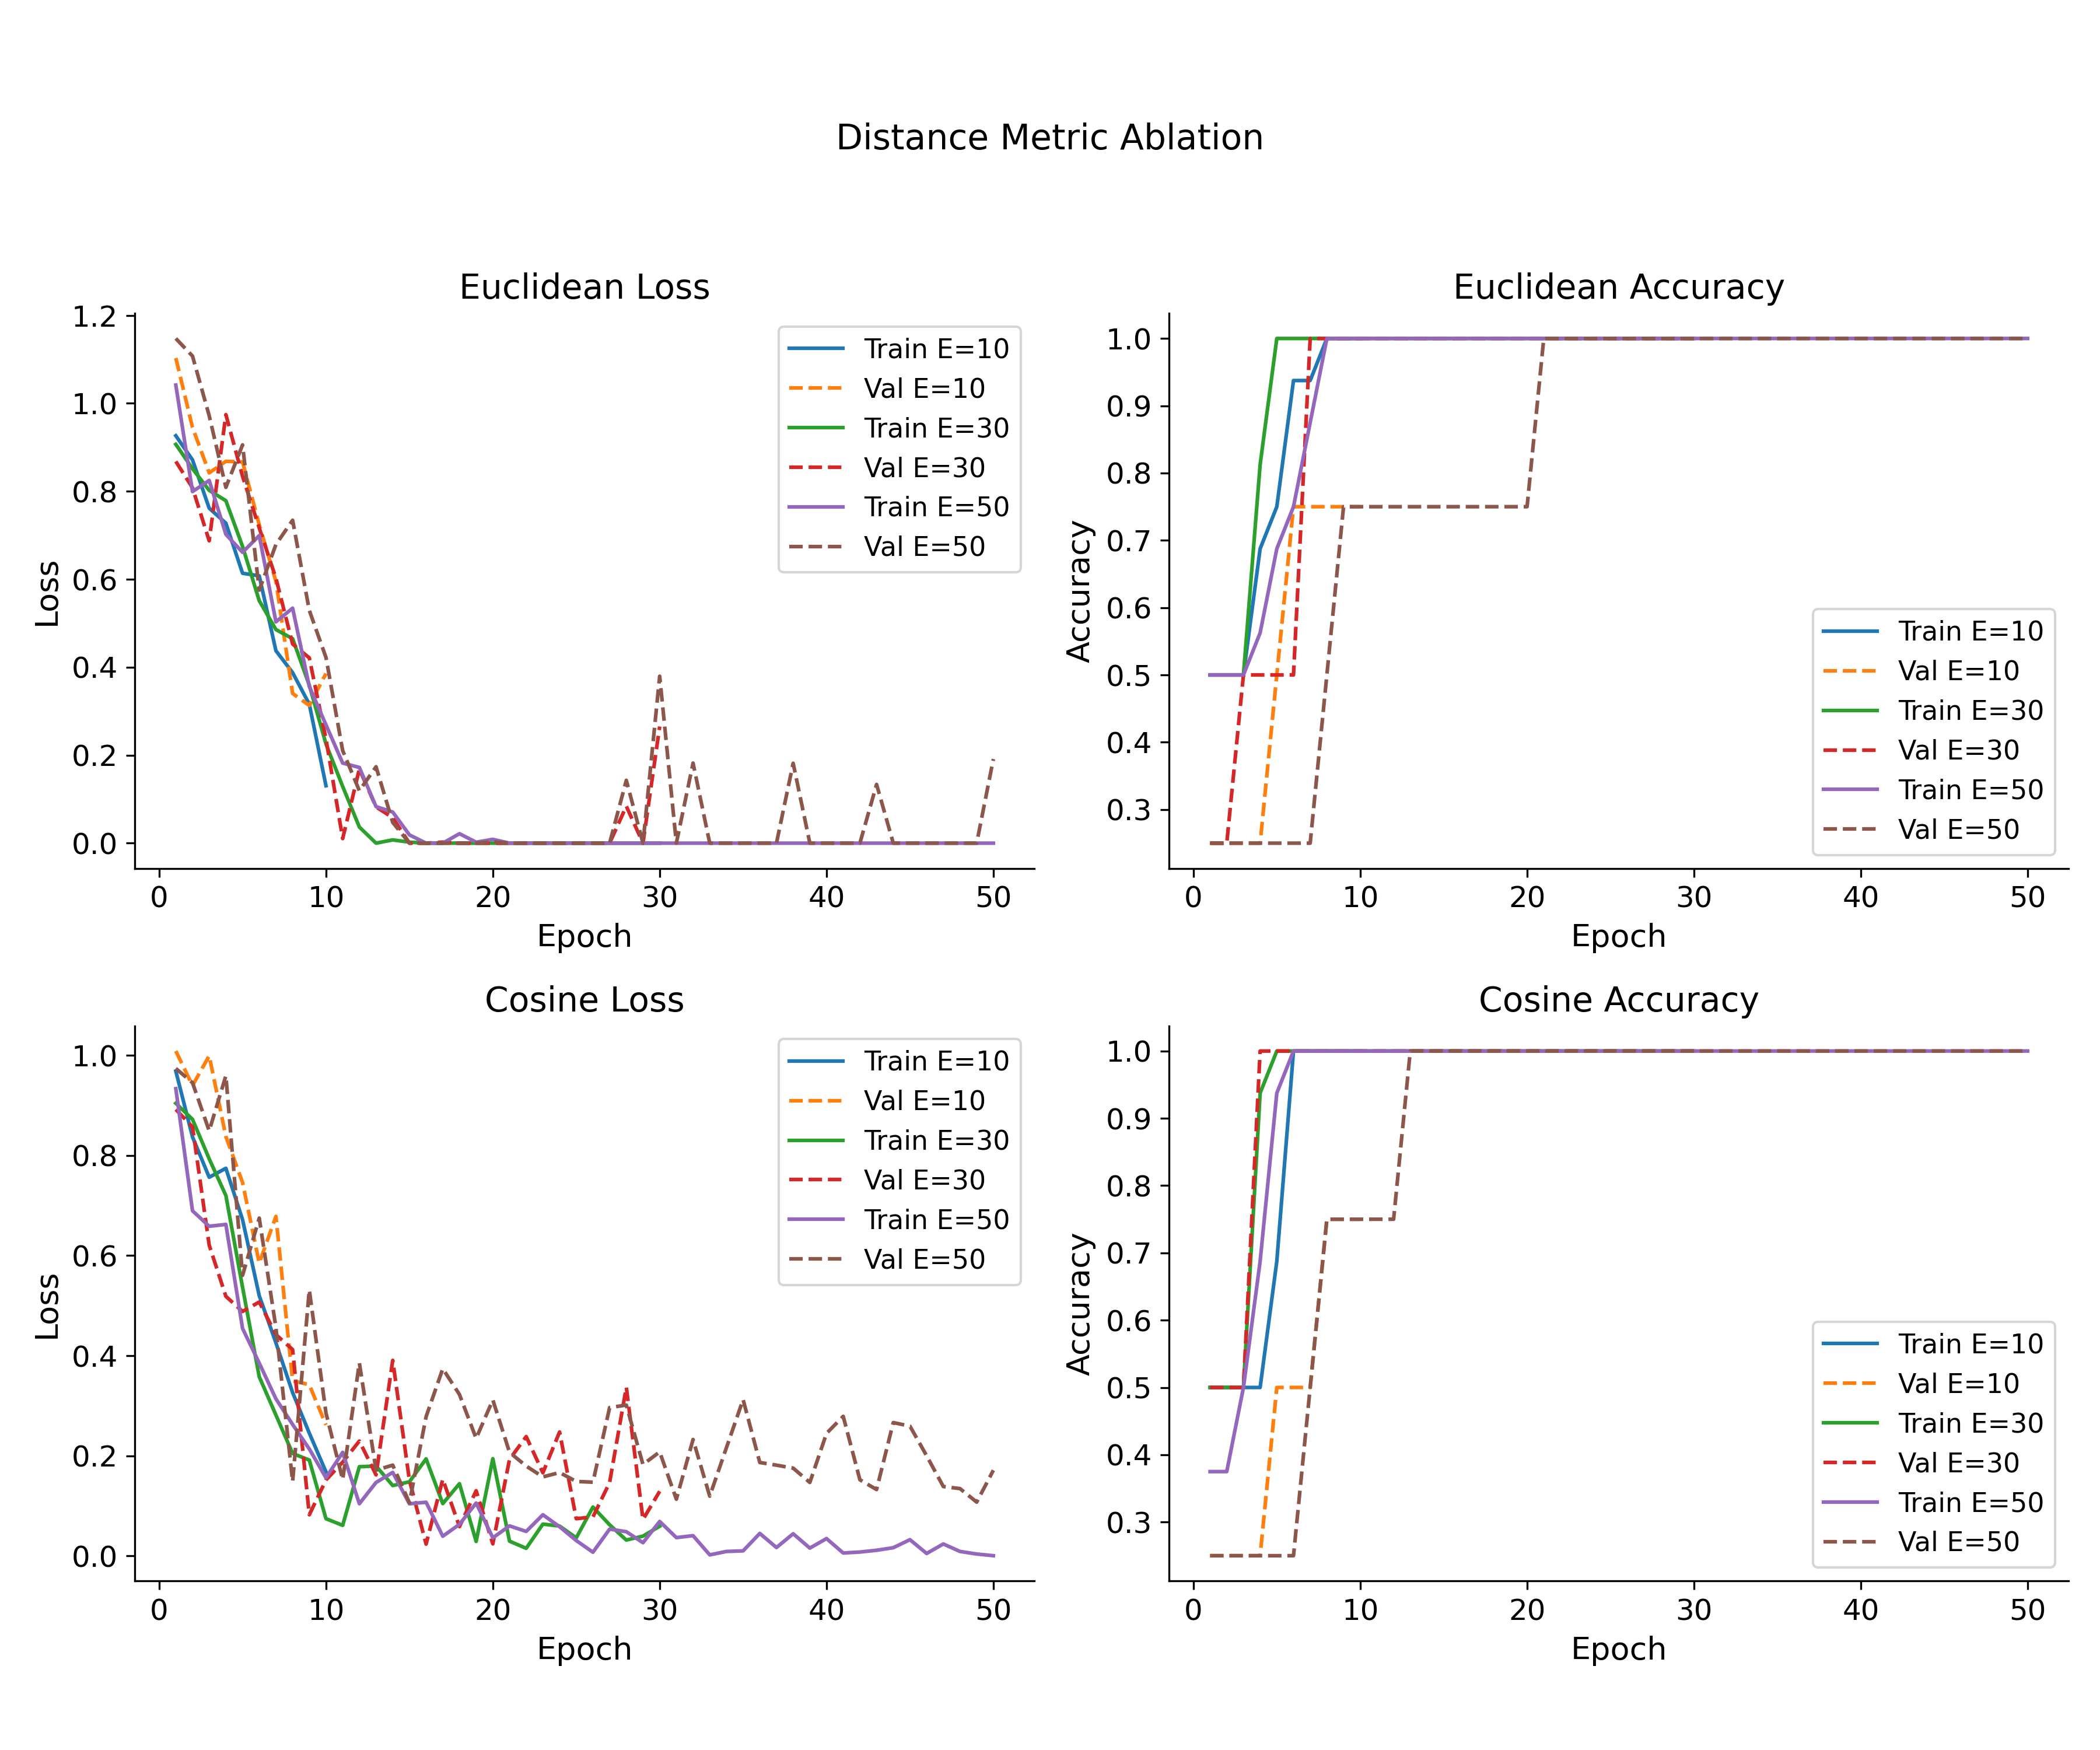
\includegraphics[width=0.9\linewidth]{distance_metric_ablation.png}
  \caption{Validation performance for Euclidean vs.\ cosine at $E=30$. Euclidean is far more stable.}
  \label{fig:dist-metric}
\end{figure}

\section{Embedding Dimension}
Figure~\ref{fig:embed-dim} highlights a capacity cliff at 64 dims: below this, validation accuracy plateaus $<0.7$; above, models saturate within 5 epochs. We recommend 64‐dim embeddings for future TraceCode pre‐training.
\begin{figure}[t]
  \centering
  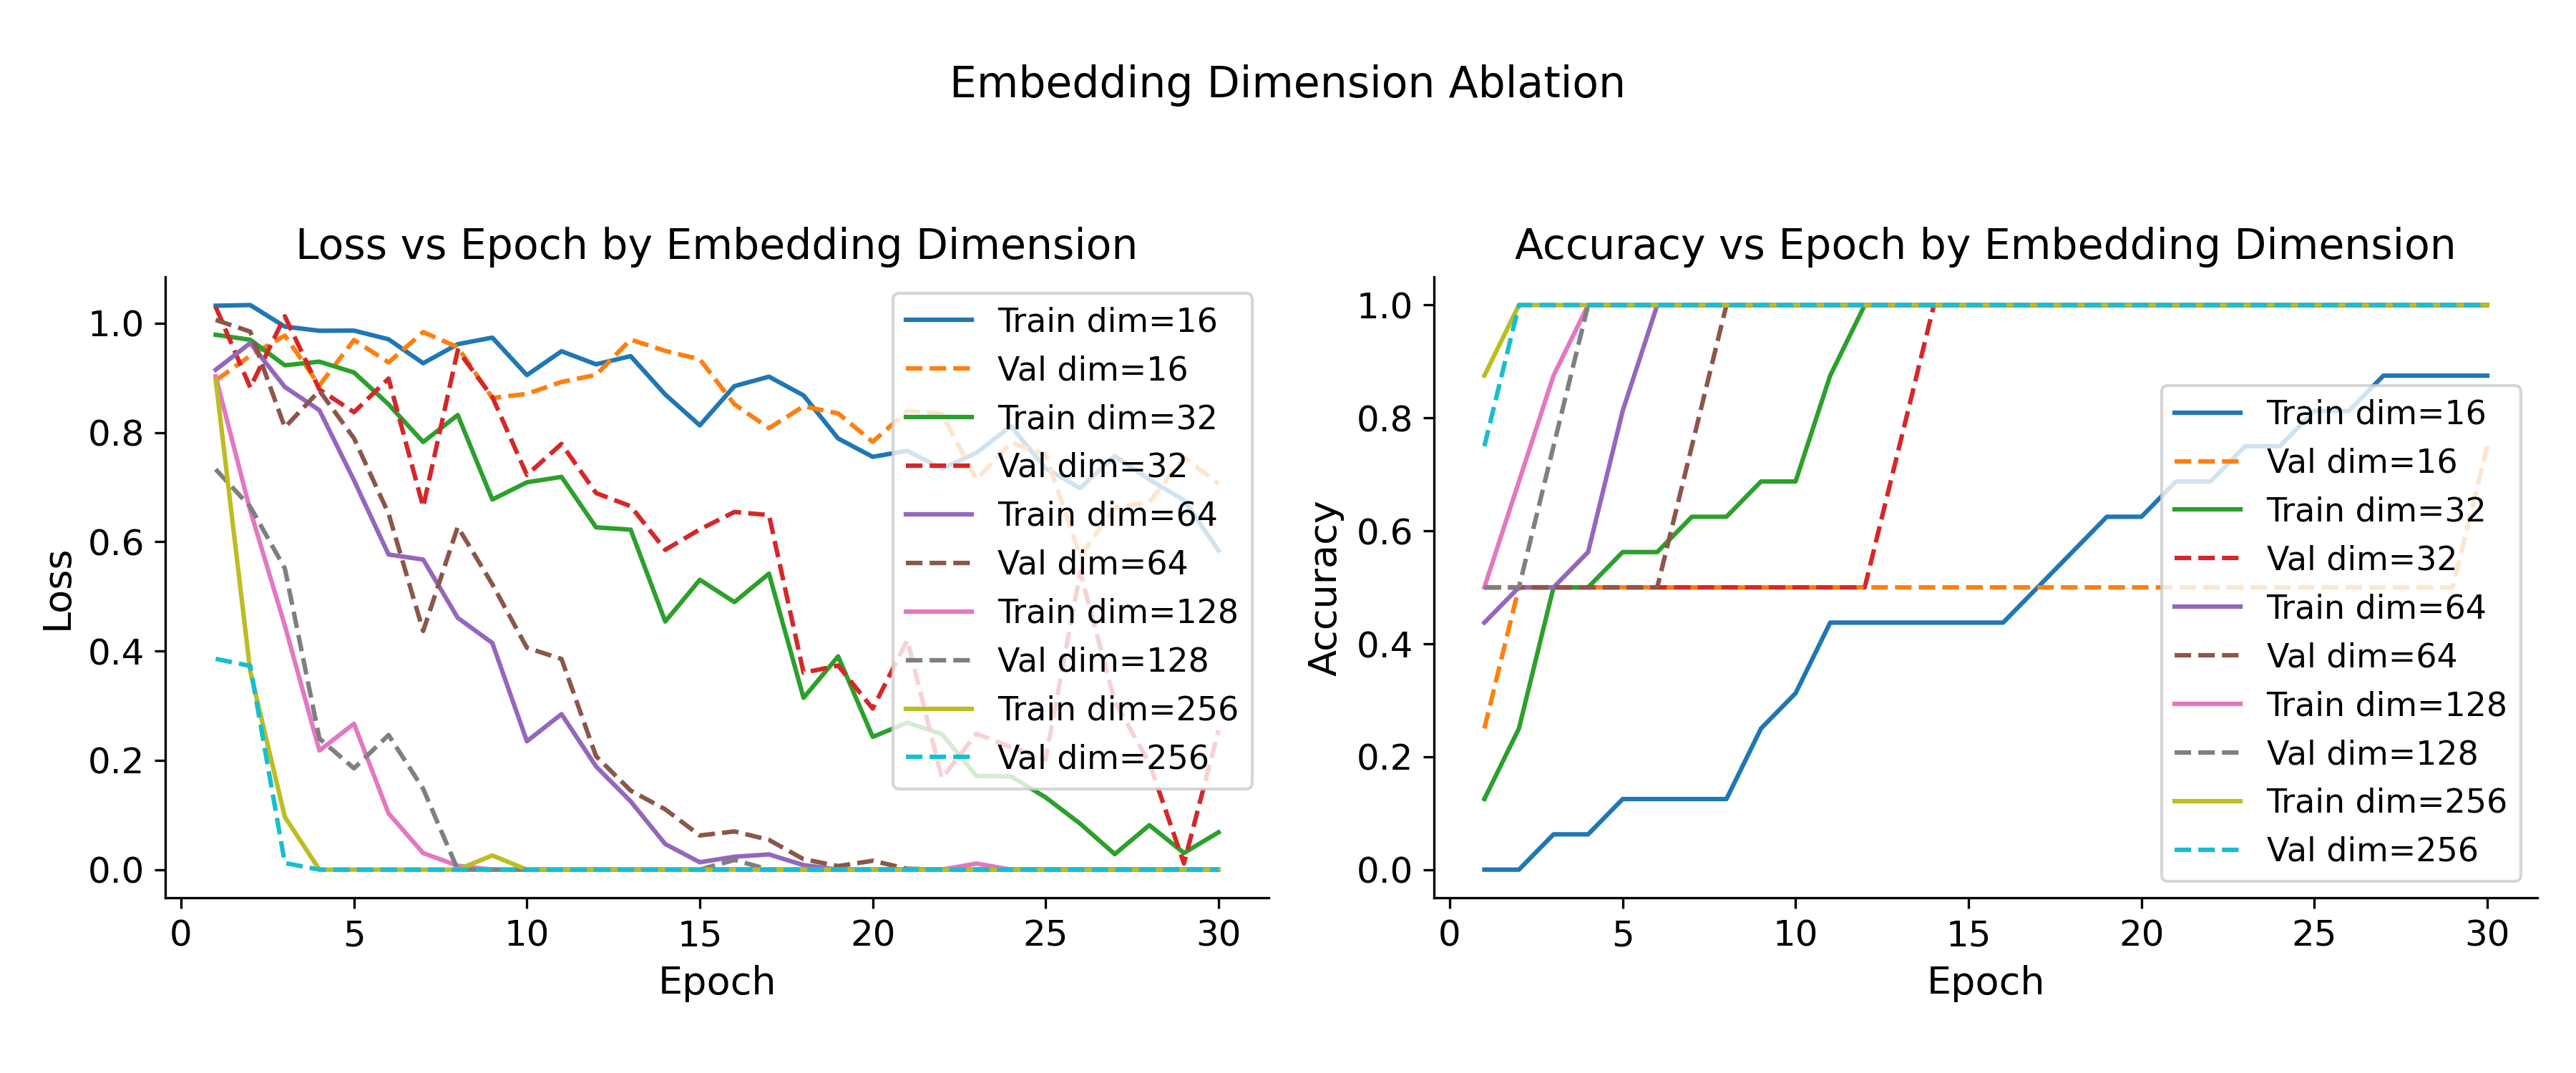
\includegraphics[width=0.9\linewidth]{embedding_dimension_ablation.png}
  \caption{Validation accuracy vs.\ embedding dimension. A clear “sweet spot” at 64 dims.}
  \label{fig:embed-dim}
\end{figure}

%%% ===== At the end of the document, before \bibliography, add the appendix =====

\appendix

\section{Appendix A: Epoch‐Budget Ablation}
\begin{figure}[h]
  \centering
  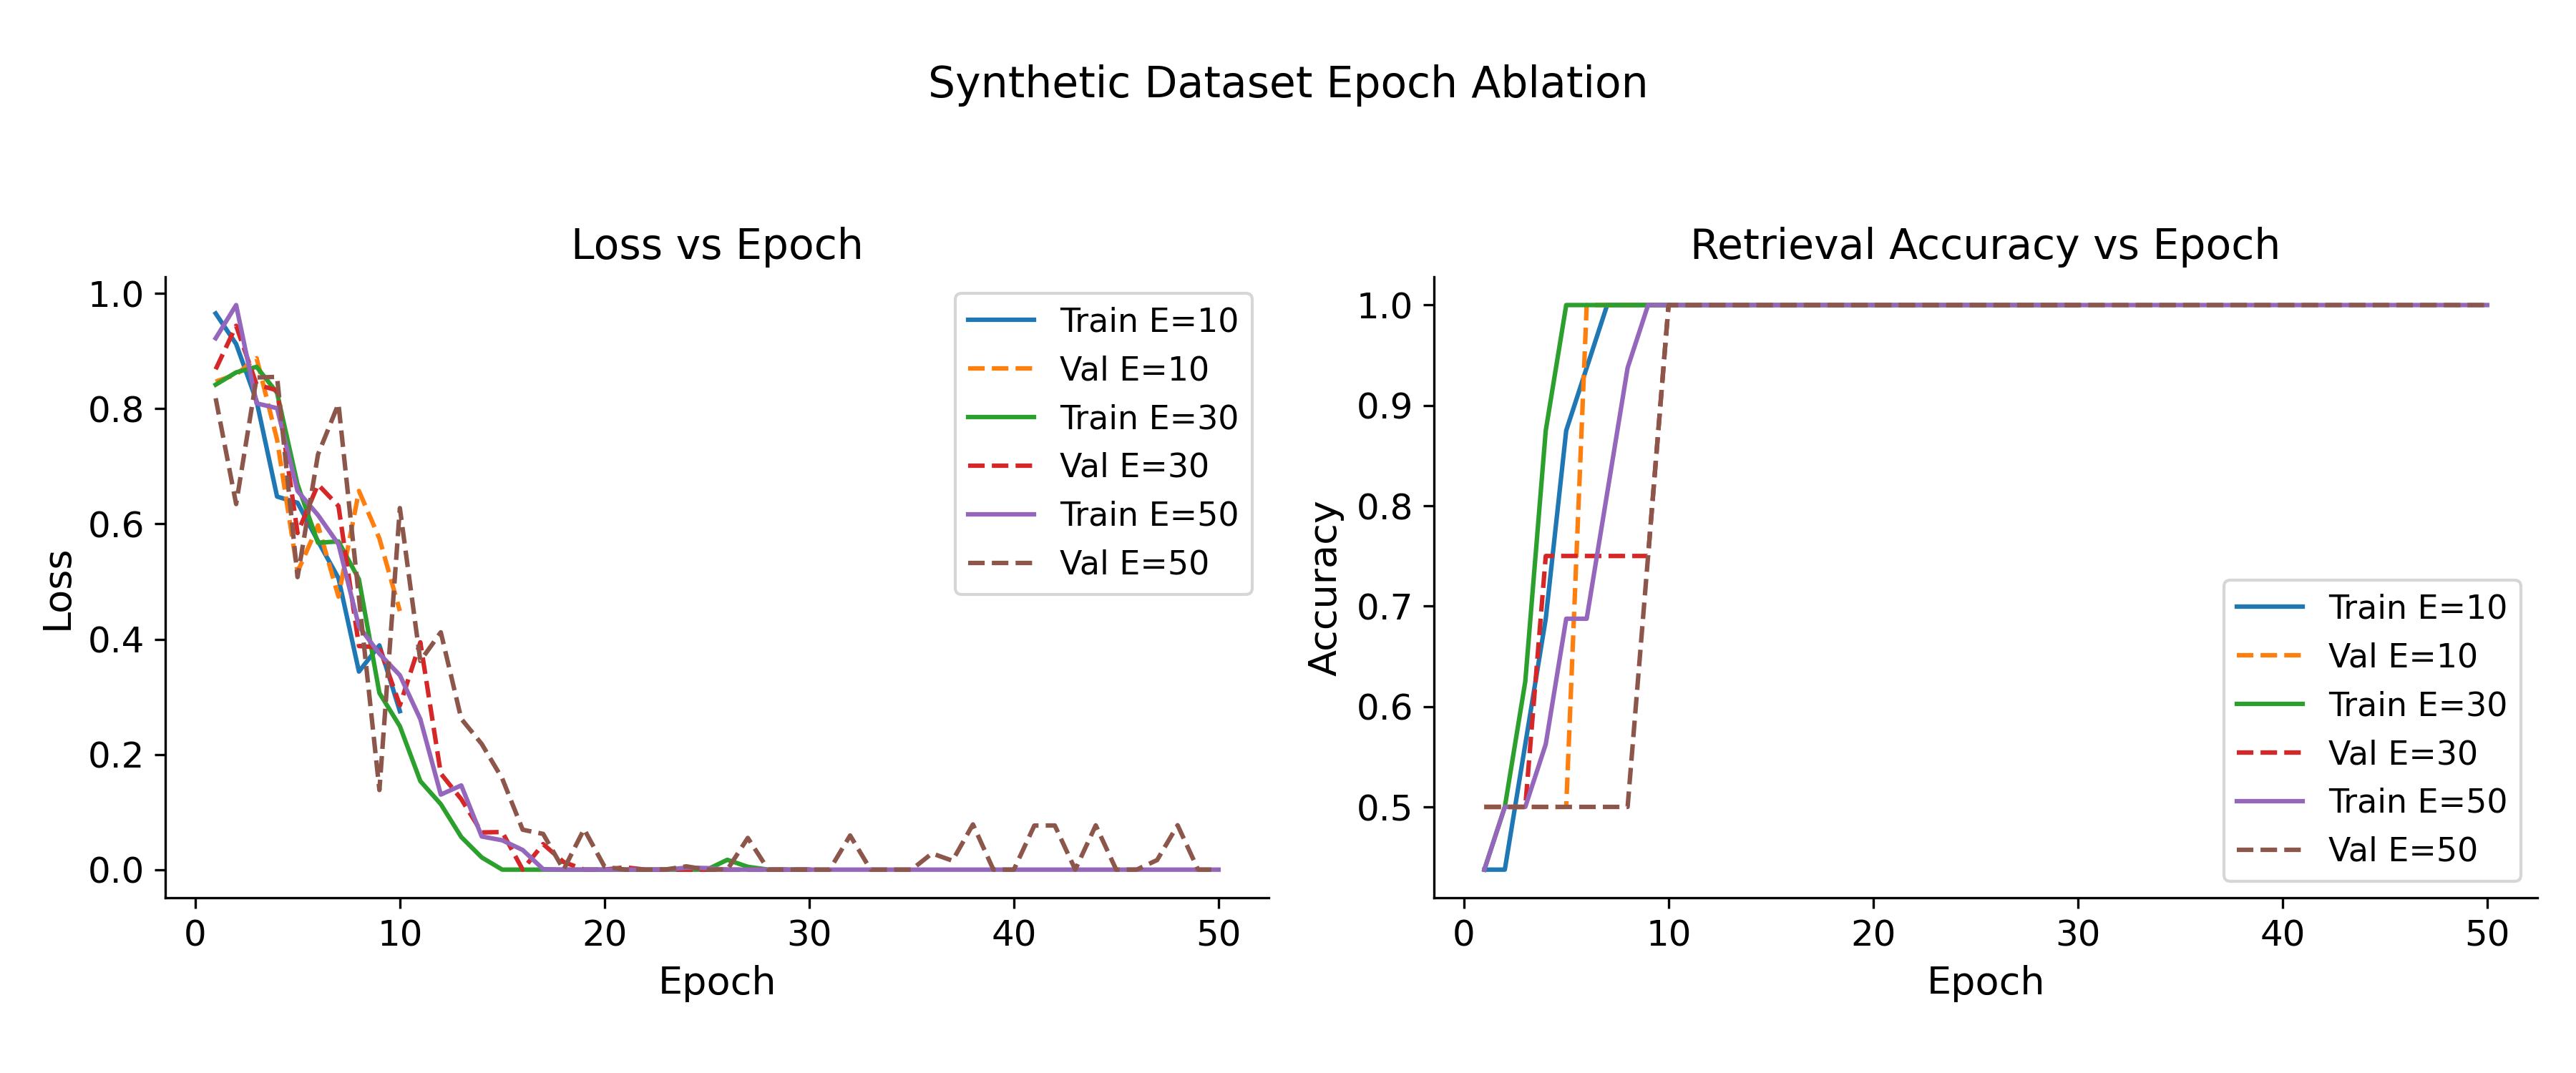
\includegraphics[width=0.9\linewidth]{synthetic_epoch_ablation.png}
  \caption{Full epoch‐budget ablation: rapid overfitting and validation spikes.}
  \label{fig:epoch-ablation-app}
\end{figure}

\section{Appendix B: Additional Ablations}
\begin{figure}[h]
  \centering
  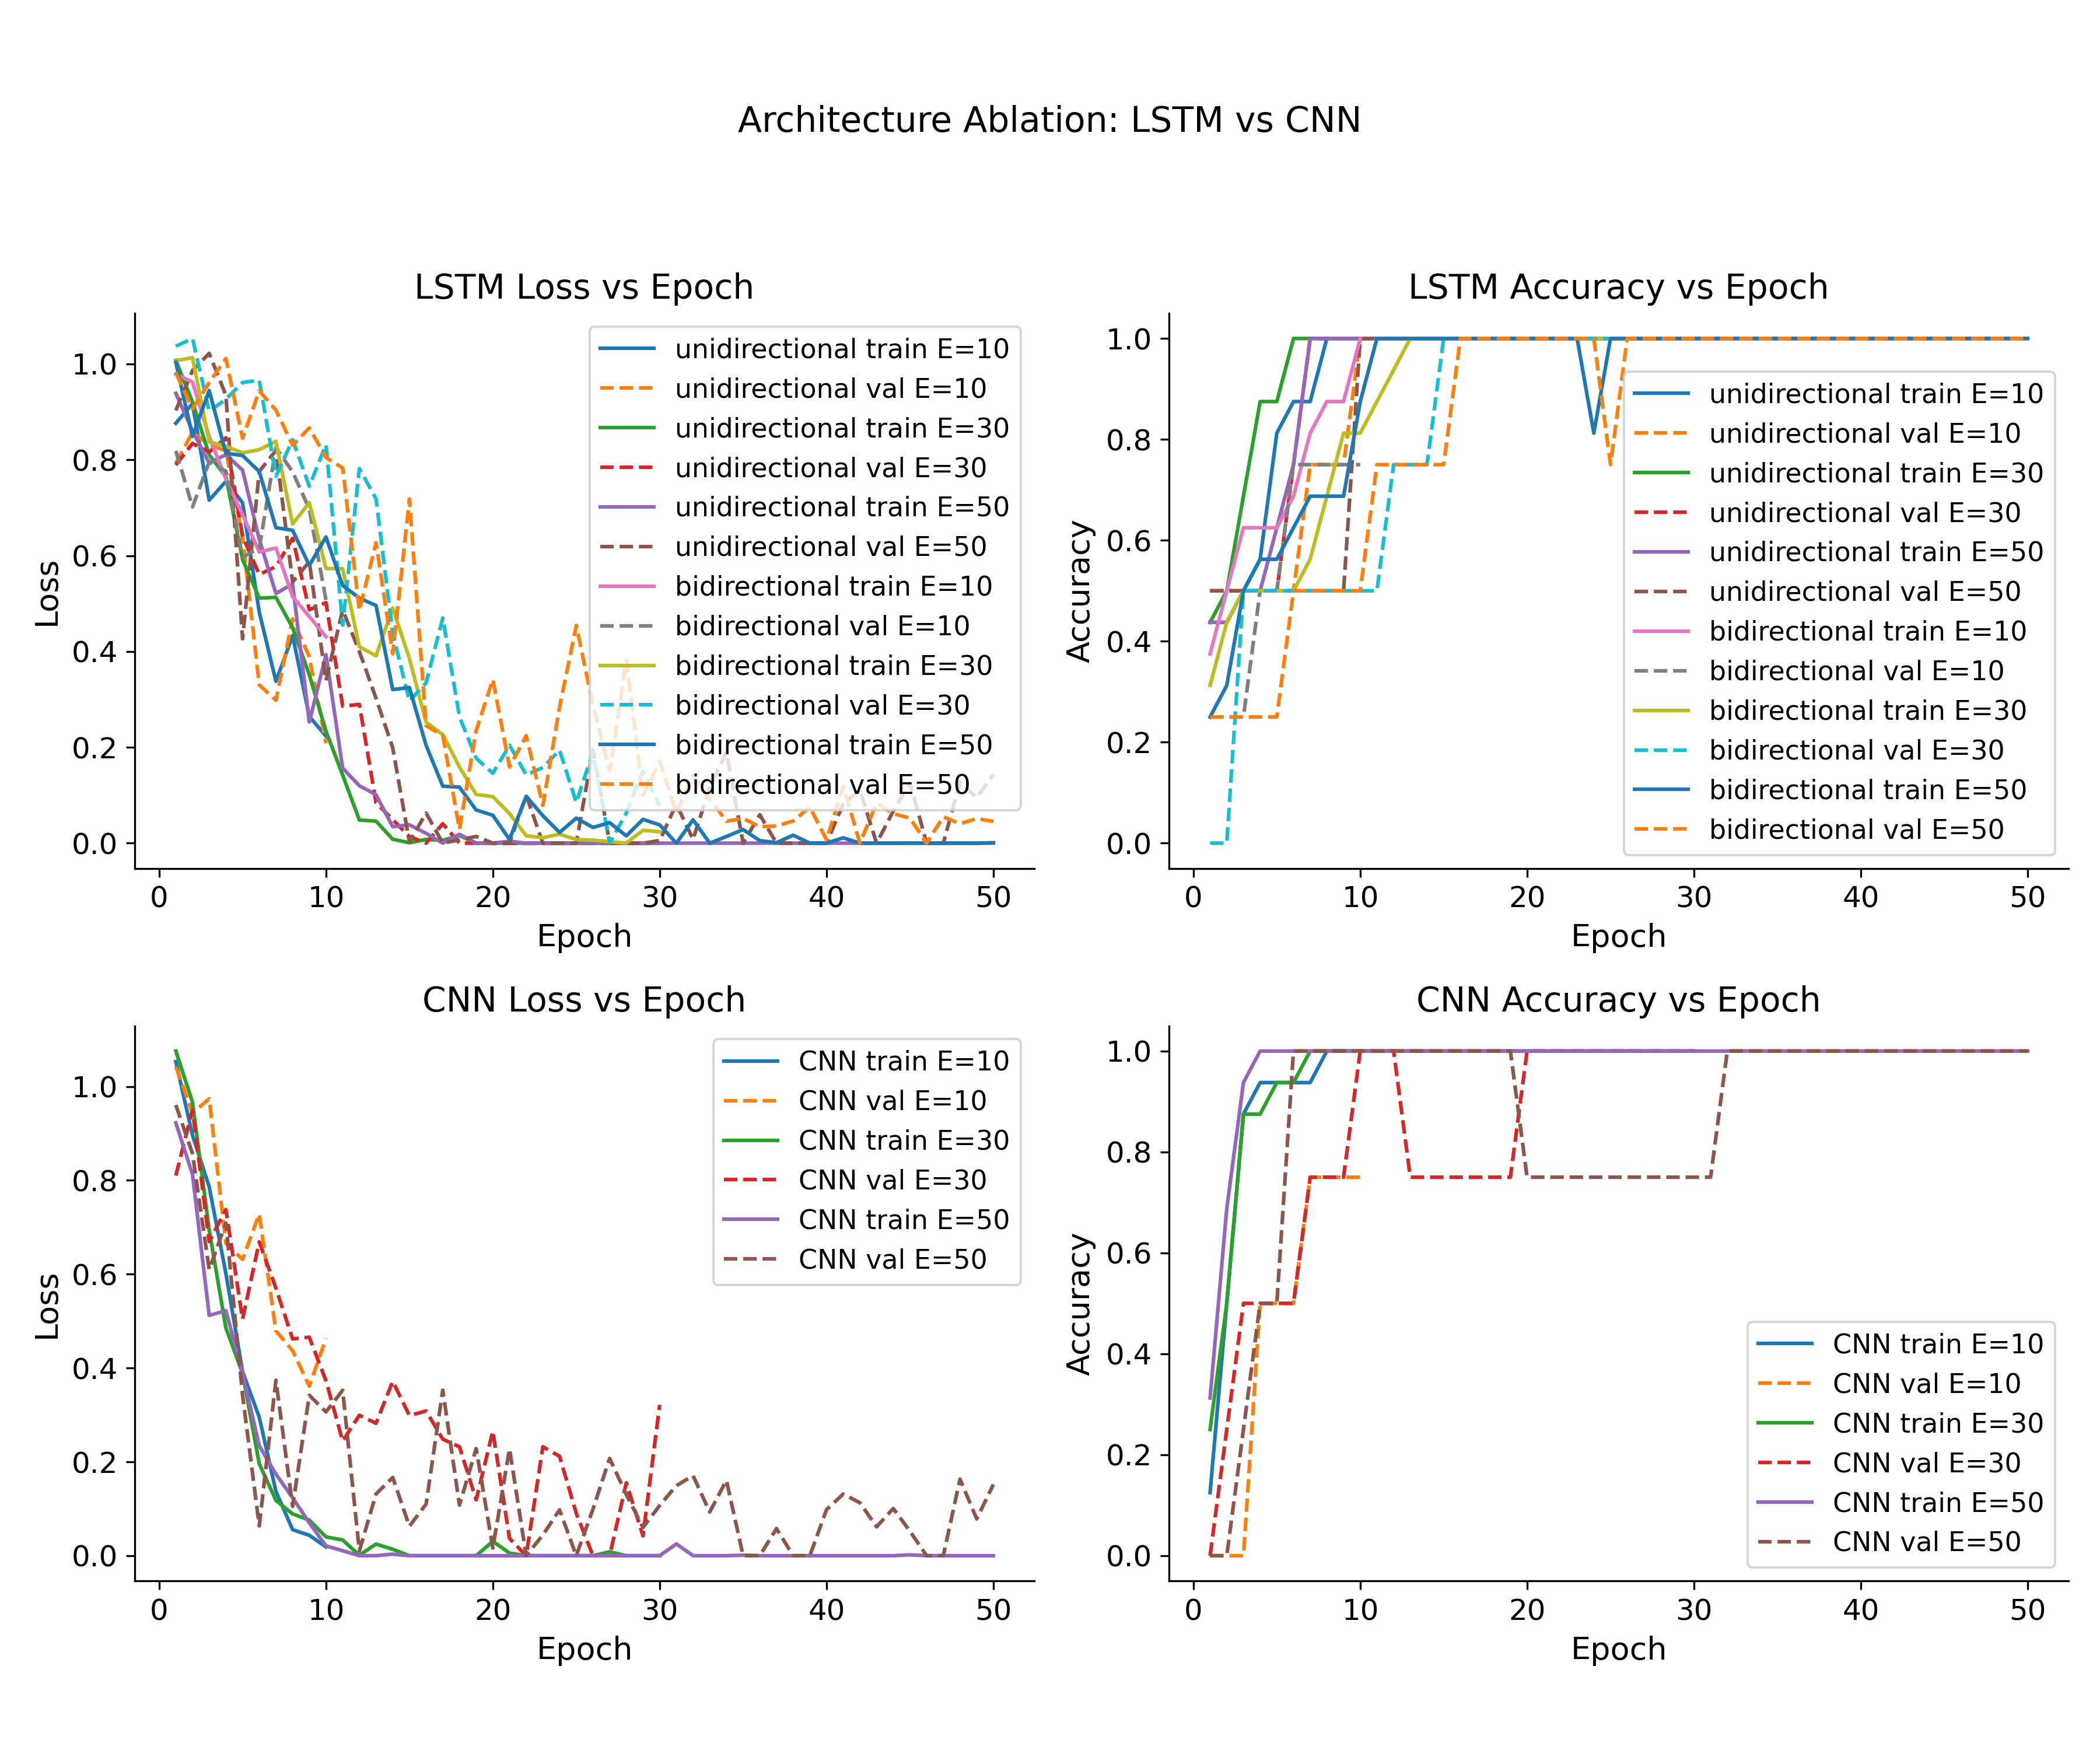
\includegraphics[width=0.48\linewidth]{architecture_ablation.png}
  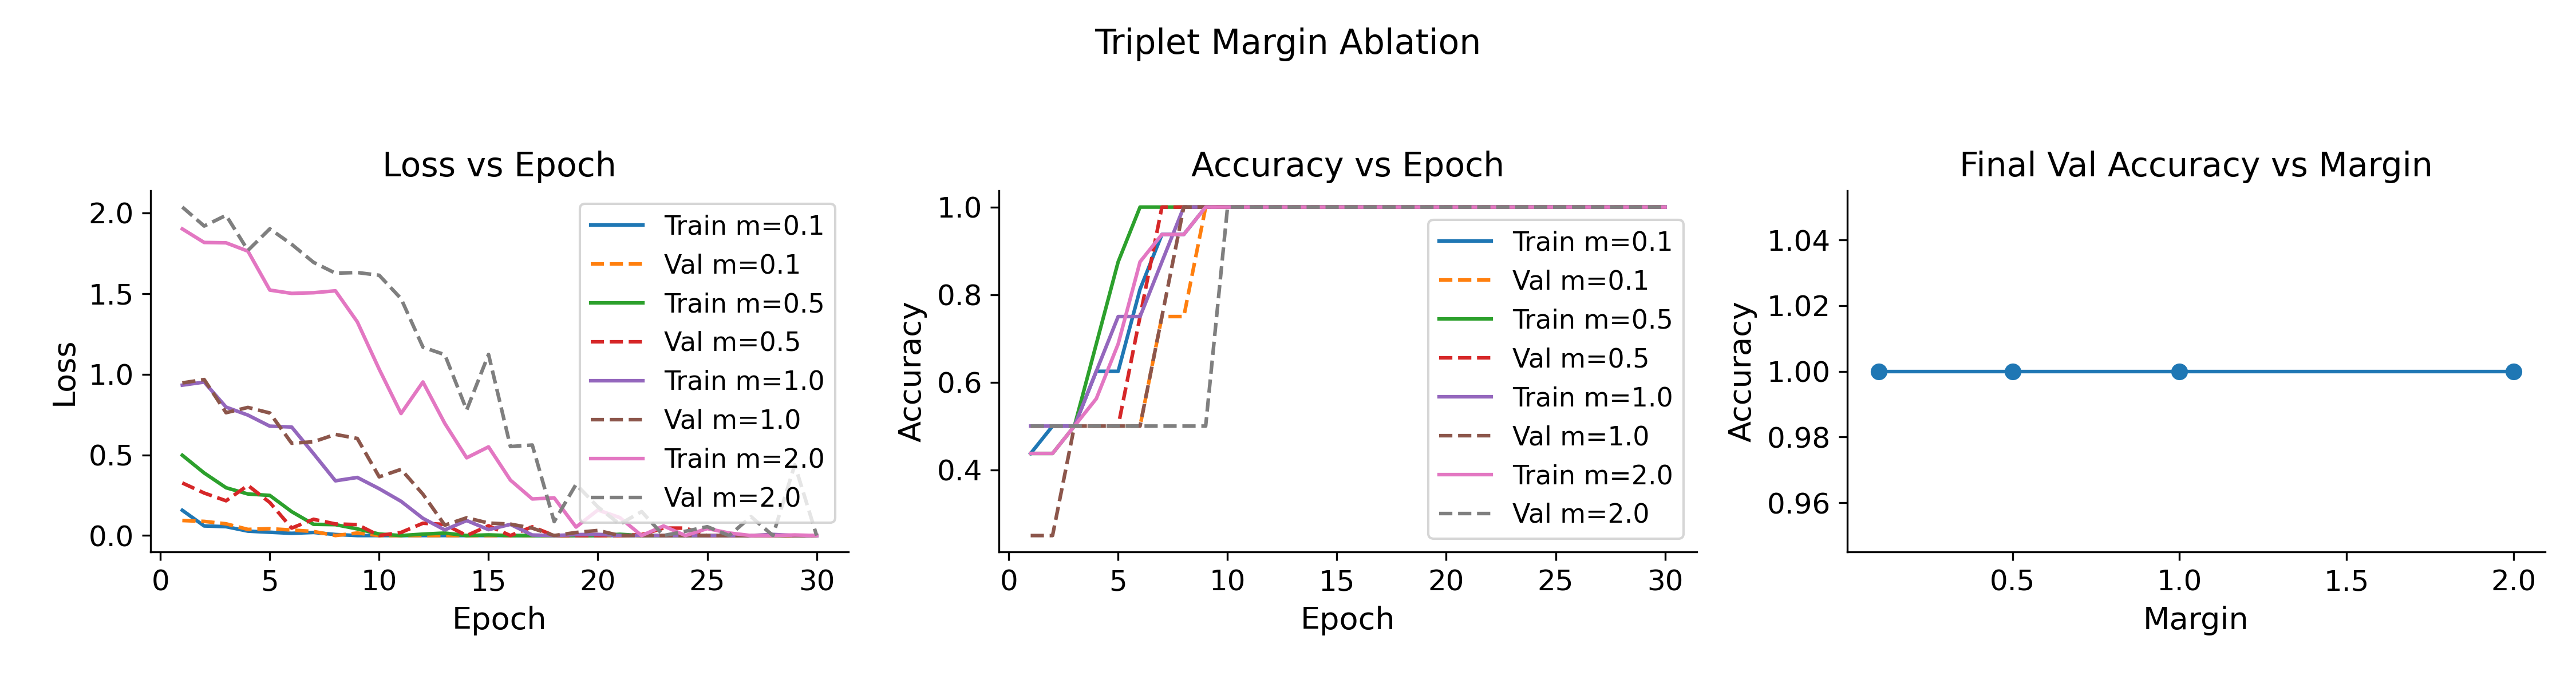
\includegraphics[width=0.48\linewidth]{triplet_margin_ablation.png}\\[1ex]
  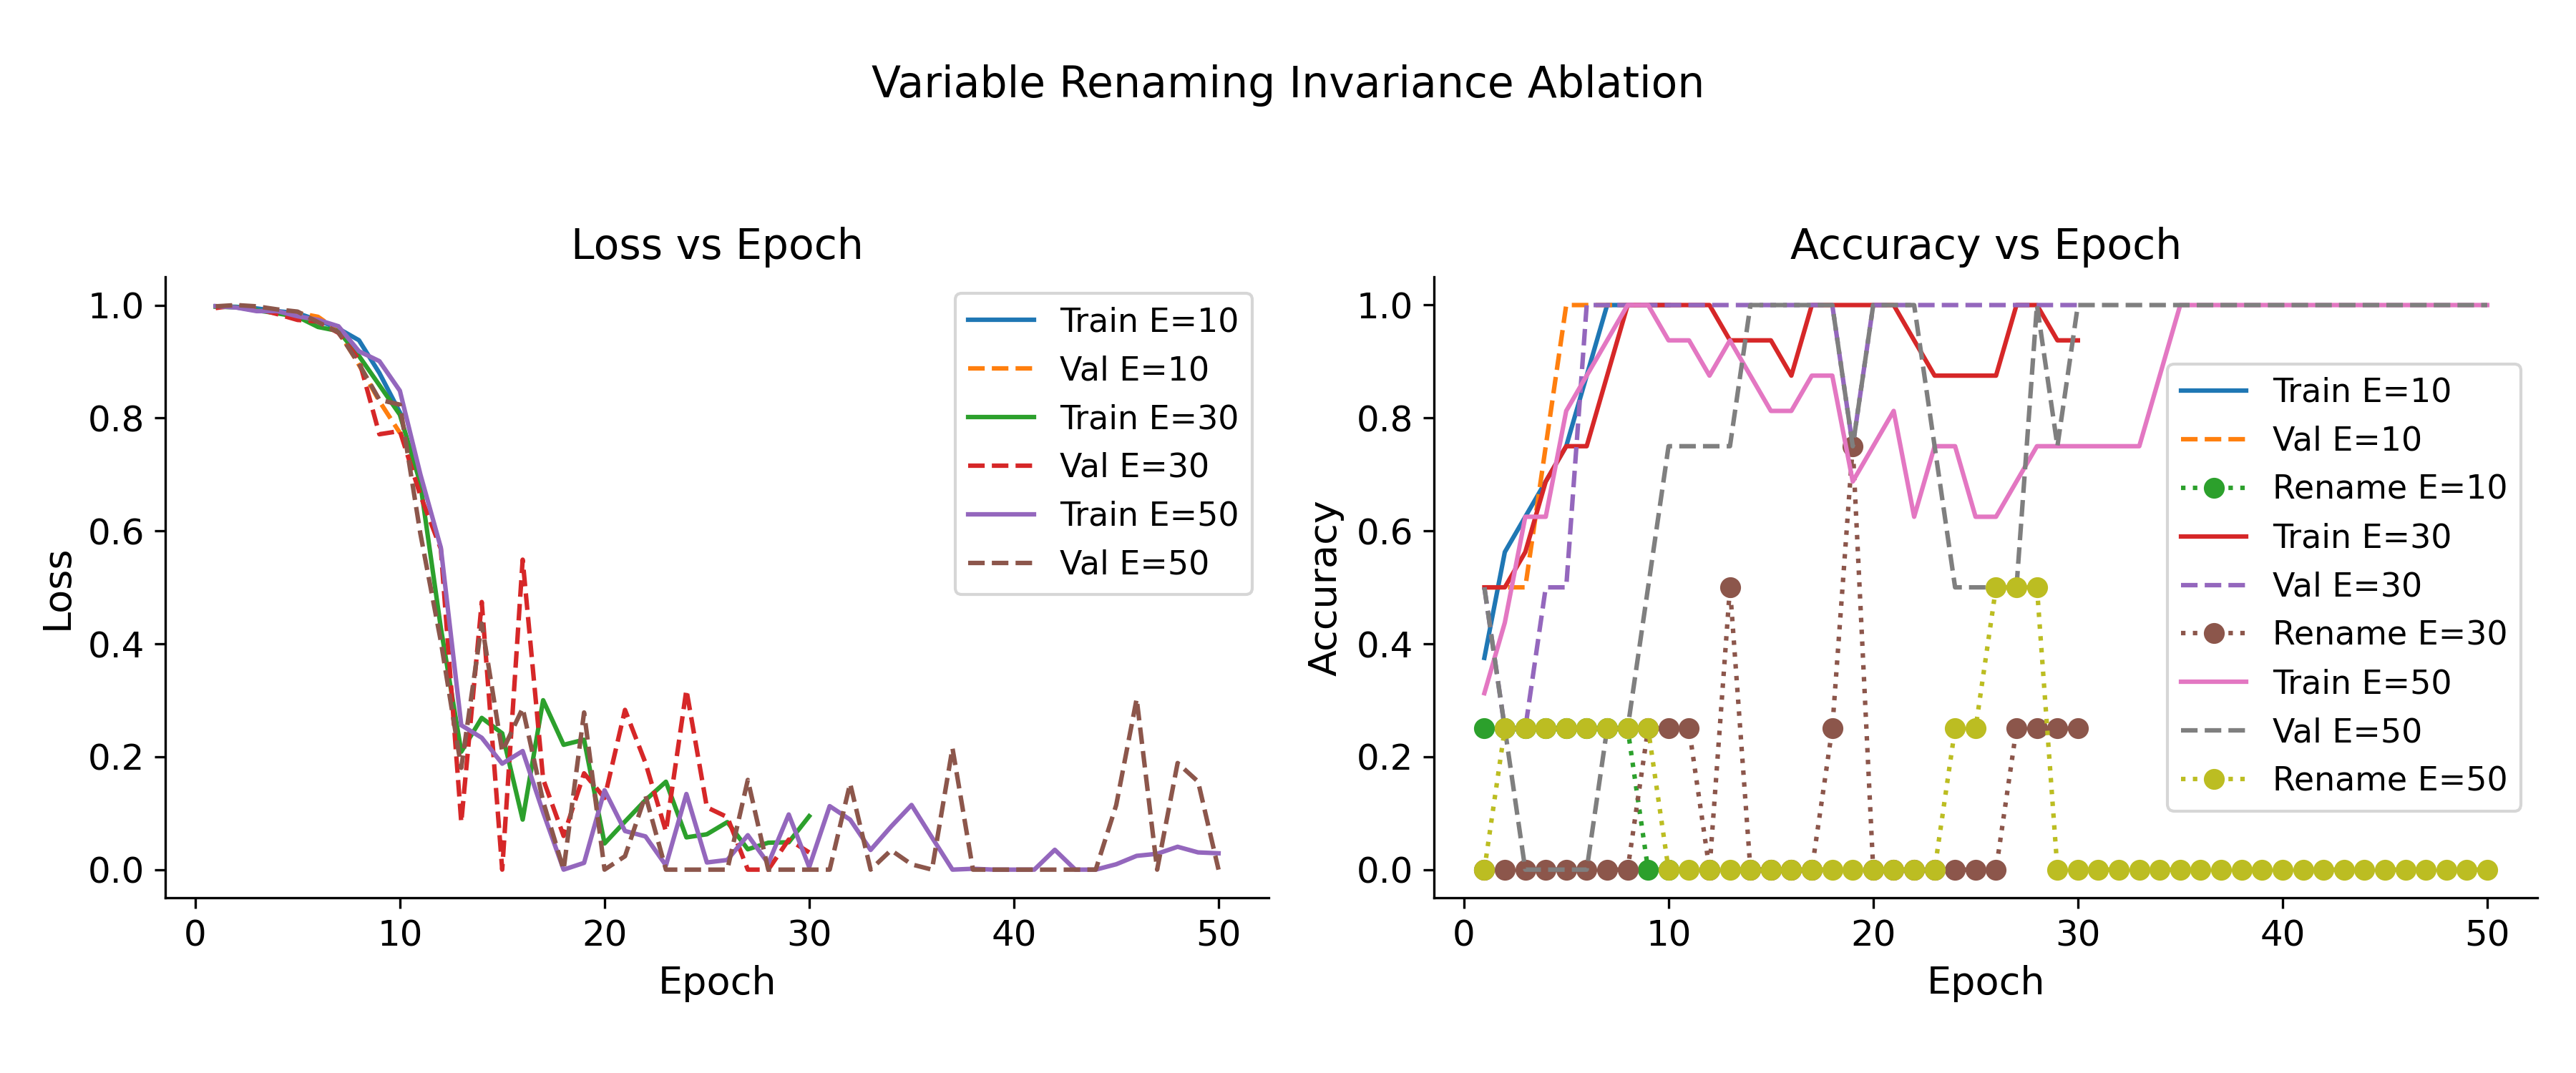
\includegraphics[width=0.48\linewidth]{variable_renaming_invariance_ablation.png}
  \caption{Additional architecture, triplet‐margin, and variable‐renaming ablations.}
  \label{fig:other-ablations}
\end{figure}

%%% ===== Remove all other \includegraphics calls from the main text. =====